
\documentclass[10pt,twocolumn]{article}
\usepackage[font=footnotesize,format=plain,labelfont=bf,up]{caption}
\usepackage{amsmath, amsfonts, amssymb}     % maths symbols
\usepackage{color, subfig}        % coloured text, subfigs
\usepackage{colortbl}                       % color in table headings
\usepackage{wrapfig}                        % not sure if needed?
\usepackage{xfrac}                          % inline fractions
\usepackage{grffile}                        % filenames with dots in

\definecolor{orange}{rgb}{1,0.5,0}
\definecolor{purple}{rgb}{0.7,0.1,1}
\definecolor{pink}{rgb}{0.9,0.1,1}

\usepackage[margin=1.1in]{geometry}


% make links to figs and refs in PDF and colour them
\usepackage[colorlinks, citecolor=blue, urlcolor=red, linkcolor=blue]{hyperref}

\renewcommand{\eqref}{Eq.~\ref}
\newcommand{\figref}{Fig.~\ref}

% macros for traces, symmetric / asymmetric parts
\newcommand{\Tr}[1] {\textrm{Tr}[#1]}
\newcommand{\SYM}[1] {[#1]^{\rm S}}
\newcommand{\ST}[1] {[#1]^{\rm ST}}

% macros for tensors / vectors
\newcommand{\tsr}[1] {\mathbf{#1}}
\newcommand{\vtr}[1] {\mathbf{#1}}
\newcommand{\uvtr}[1] {\hat{\mathbf{#1}}}
\newcommand{\dd}[2] {\frac{\partial #1}{\partial #2}}
\newcommand{\gdot}[0] {\dot{\gamma}}
\newcommand{\gdotb}[0] {\bar{\dot{\gamma}}}
\newcommand{\degree}{\ensuremath{^\circ}}
\newcommand{\params}{\textbf{Parameters: }}
\newcommand{\inset}{\textbf{Inset: }}

\newcommand{\etal}{\textit{et al.} }
\newcommand{\note}[1] {(\textcolor{red}{\textit{#1}})}

\begin{document}

\title{Elastic Turbulence}
\author{Ewan Hemingway, Suzanne Fielding}

\date{\today}

\maketitle

\section{Results}

In \cite{Thomases2007}, Thomases and Shelly solve Oldroyd B in a four-mill fixed flow, studying the dynamics as a function of $Wi = \frac{\tau}{\tau_f}$ where $\tau_f$ is a timescale set by the forcing.

In \cite{Thomases2011}, they include a diffusive term keeping stress bounded.

\begin{figure*}
  \centering
  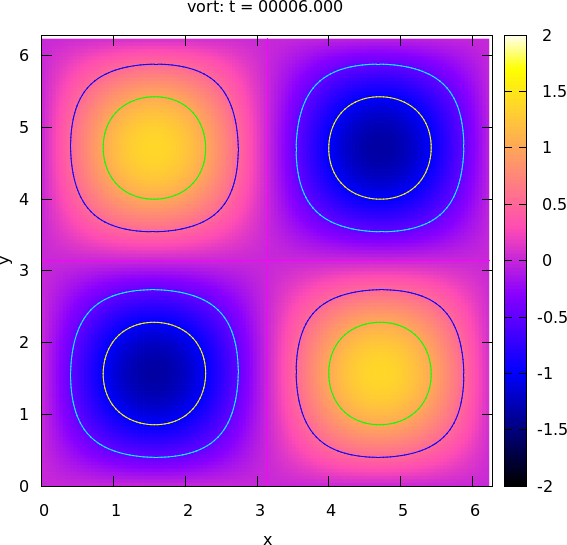
\includegraphics[width=0.3\textwidth]{images/vort_Wi0.3.png}
  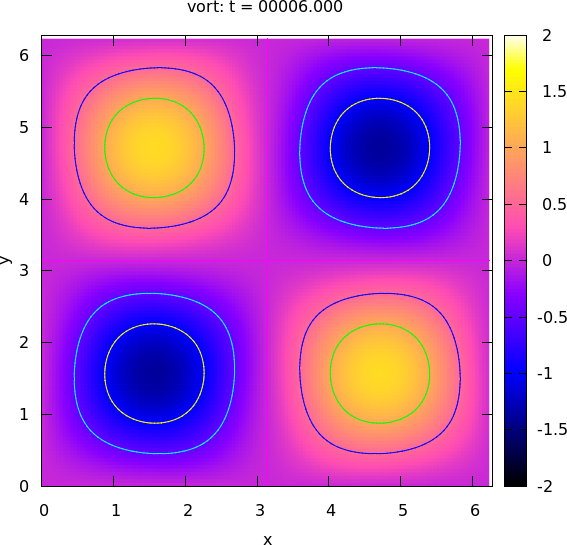
\includegraphics[width=0.3\textwidth]{images/vort_Wi0.6.png}
  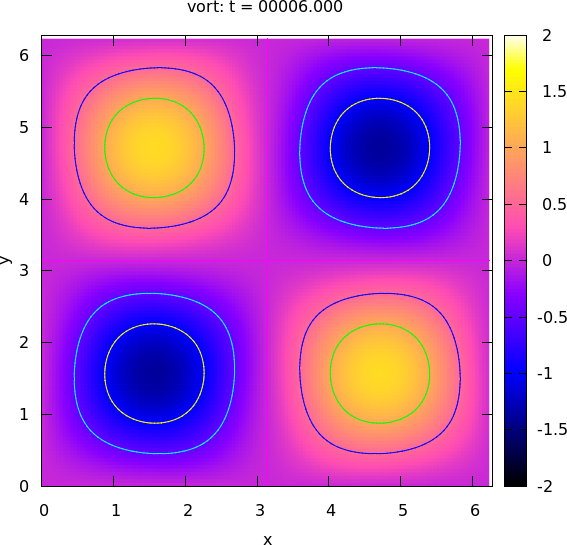
\includegraphics[width=0.3\textwidth]{images/vort_Wi0.6.png}

  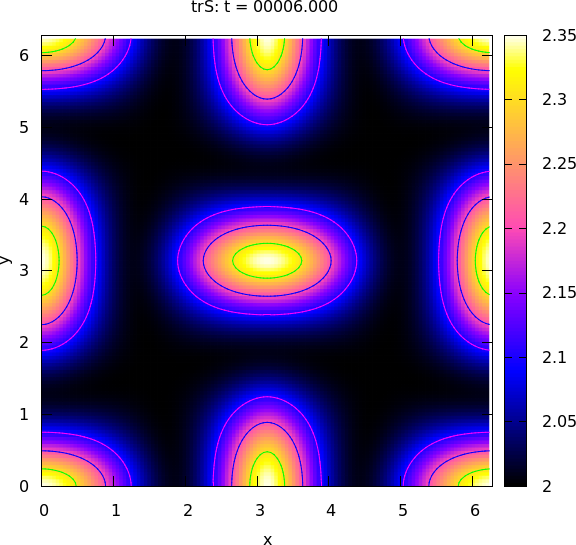
\includegraphics[width=0.3\textwidth]{images/trS_Wi0.3.png}
  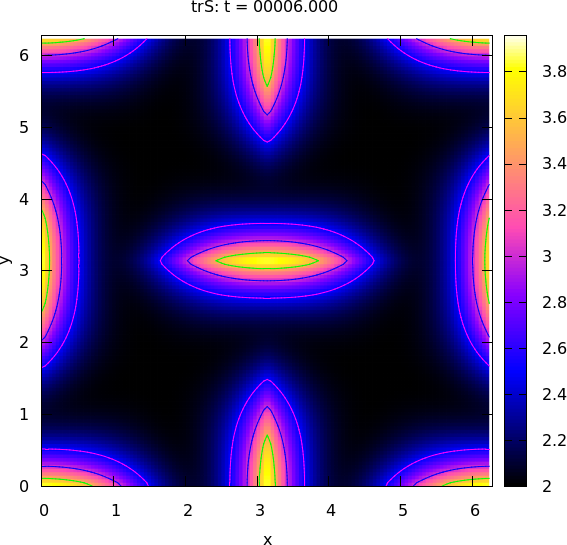
\includegraphics[width=0.3\textwidth]{images/trS_Wi0.6.png}
  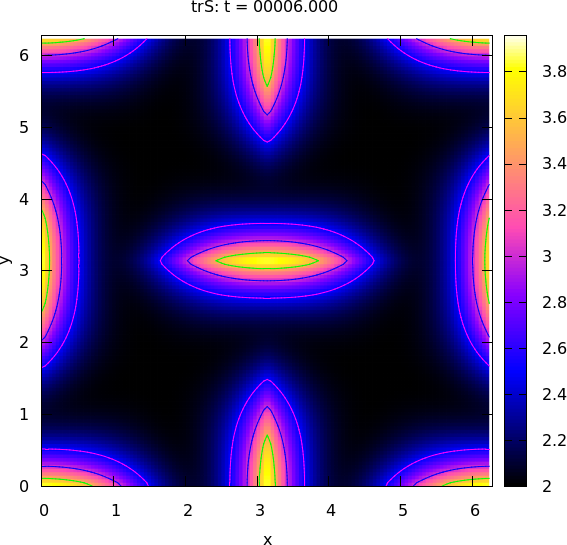
\includegraphics[width=0.3\textwidth]{images/trS_Wi0.6.png}
  \caption{dh}
  \label{fig:without_diffusion}
\end{figure*}




%\clearpage
%\section{Parameters}
%\label{apx:parameters}

%Table \ref{tbl:params} lists all model parameters, and includes our choice of units. We distill this down to four dimensionless parameters, one of which ($\chi$) is zero for the majority of the study (Table \ref{tbl:params_dimensionless}).
%\begin{table*}
  %\def\arraystretch{1.5}
  %\begin{center}
    %\begin{tabular}{| l | l | l | l |}
      %\hline
      %\rowcolor[gray]{.5}\textbf{parameter} & \textbf{dimensions} & \textbf{value} & \textbf{description}\\
      %\hline \multicolumn{4}{|c|}{\textbf{system (or shared) parameters}}\\ \hline
      %$\rho$ & [$ML^{-3}$] & 0 (\textcolor{red}{fixed})& density\\
      %$\eta$ & [$ML^{-1}T^{-1}$] = [$GT$] & 0.567 (\textcolor{red}{fixed}) & solvent viscosity\\
      %$L_x$ & [$L$] & 4 (\textcolor{red}{fixed}) & box size (in periodic direction)\\
      %\rowcolor[gray]{.7}$L_y$ & [$L$] & 1 (\textcolor{red}{fixed}) & box size (distance between walls)\\
      %$\Delta x$, $\Delta y$ & [$L$] & converge $\to 0$ & space-step\\
      %$\Delta t$ & [$T$] & converge $\to 0$ & time-step \\

      %\hline \multicolumn{4}{|c|}{\textbf{active nematic parameters} ($\tsr{Q}$)}\\ \hline
      %\rowcolor[gray]{.7}$G_Q$ & [G] & 1 (\textcolor{red}{fixed})& $\tsr{Q}$ modulus (appears in bulk FE) \\
      %\rowcolor[gray]{.7}$\tau_Q$ & [T] & 1 (\textcolor{red}{fixed})& $\tsr{Q}$ relaxation time \\
      %$\gamma$ & [1] & 3 (\textcolor{red}{fixed}) & isotropic-nematic control param.\\
      %$\xi$ & [1] & 0.7 (\textcolor{red}{fixed}) & flow aligning ($\xi > \sfrac{3}{5}$) \\
      %$\zeta$ & $[ML^{-1}T^{-2}] = [G]$ & 0.001$\to$ 10  (\textcolor{green}{vary}) & extensile activities ($\zeta > 0$)\\
      %$\ell_Q = \sqrt{\frac{K}{G_Q}} $ & [$L$] & $0.002 \to 0.025$  (\textcolor{green}{vary $\Delta = \frac{\ell_Q^2}{\tau_C} = \frac{\ell_C^2}{\tau_C}$})&Frank length\\

      %\hline \multicolumn{4}{|c|}{\textbf{polymer parameters} ($\tsr{C}$)}\\ \hline
      %$G_C$ & [G] & $\sfrac{\eta_C}{\tau_C}$  (\textcolor{blue}{slaved by constraint $\eta_C = 1$})& $\tsr{C}$ modulus \\
      %$\tau_C$ & [T] & $10^{-2}\to10^6 \to \infty$ (\textcolor{green}{vary})& $\tsr{C}$ relaxation time \\
      %$\ell_C$ & [L] & $\frac{\ell_Q^2}{\tau_Q} =\frac{\ell_C^2}{\tau_C} = \Delta$ (\textcolor{blue}{slaved to $\ell_Q$})& diffusive lengthscale \\
      %$a$ & [1] & 1 (\textcolor{red}{fixed}) & slip param ($a=1$ is Oldroyd B)\\

      %\hline \multicolumn{4}{|c|}{\textbf{explicit coupling parameters} ($\tsr{Q} + \tsr{C}$)}\\ \hline
      %$\chi$ & $[G]$ & $\chi \ll G_Q, G_C$ (\textcolor{green}{vary}) or 0 (\textcolor{red}{fixed})& \\
      %$\kappa$ & $[G]$ & 0 (\textcolor{red}{fixed}) & \\
      %\hline
    %\end{tabular}
    %\caption{List of model parameters, \textbf{grey} rows show our choice for units of length $[L]$, modulus $[G]$, and time $[T]$ respectively.}
    %\label{tbl:params}
  %\end{center}
%\end{table*}

%\begin{table*}
  %\def\arraystretch{1.5}
  %\begin{center}
    %\begin{tabular}{| l | l | l |}
      %\hline
      %\rowcolor[gray]{.5}\textbf{parameter} & \textbf{value} & \textbf{description}\\
      %$\tilde{\zeta} = \sfrac{\zeta}{G_Q}$ &  0.001$\to$ 10 & activity ($\zeta > 0$)\\
      %$\tilde{\Delta} \equiv \frac{K}{G_Q L_y^2} $ & $10^{-5} \to 6.4 \times10^{-4}$ & diffusive constant \\
      %$\tilde{\tau}_C \equiv \sfrac{\tau_C}{\tau_Q}$ & $10^{-2}\to10^6 \to \infty$ & polymer relaxation time \\
      %$\tilde{\chi} \equiv \sfrac{\chi}{G_Q}$ & $\chi \ll G_Q, G_C$ or 0 & explicit coupling strength\\
      %\hline
    %\end{tabular}
    %\caption{List of dimensionless parameters which we vary. We drop tildes for clarity.}
    %\label{tbl:params_dimensionless}
  %\end{center}
%\end{table*}


%\section{Limiting cases}

%Our choice of $\frac{\ell_Q^2}{\tau_Q} = \frac{\ell_C^2}{\tau_C} = \Delta$ means that the stability criteria \eqref{eq:criteria_zeta_full} can also can be written (note $\tau_C$ in the denominator)

%\begin{align}
  %\zeta_c = \frac{12 k^2 \Delta}{\Lambda}\left[\eta + \frac{\Lambda^2}{72}\eta_Q + \frac{a^2\tau_C G_C }{1 + k^2\Delta\tau_C} \right].
%\end{align}

%Taking $\tau_C\to\infty$ with $G_C$ fixed leads to

%\begin{align}
  %\lim_{\tau_C \to \infty} \zeta_c &= \frac{12 k^2 \Delta}{\Lambda}\left[\eta + \frac{\Lambda^2}{72}\eta_Q + \frac{a^2\tau_C G_C }{1 + k^2\Delta\tau_C} \right]\\
  %&= \frac{12 k^2 \Delta}{\Lambda}\left[\eta + \frac{\Lambda^2}{72}\eta_Q + \frac{a^2 G_C }{k^2\Delta} \right].
%\end{align}

%In the infinite system size limit \( k \to 0 \), this becomes

%\begin{align}
  %\lim_{q \to 0} \zeta_c &= \frac{12 a^2 G_C  }{\Lambda},
%\end{align}

%\noindent which oddly suggests the bulk instability is suppressed for infinite $\tau_C$. Underhill see this for finite $\eta_C$ \cite{Bozorgi2013}, though this could just be a limit in which the stability analysis breaks down.

\bibliographystyle{apsrev}
\bibliography{$HOME/papers/bibtex/library,$HOME/papers/books}

\end{document}
